% Consolidated 37-molecules-crystals from 3014fceb998eba4990e2b4a247494872c4c8e1cc; original TeX fragments preserved.

% === BEGIN 37-molecules-crystals-167-180.tex blob 8ecabb00edcb3eace7b4de6bc1d5e21be08f55ec ===
% 原书第六篇6.4节：分子与晶体167--180题。
% 底本 Irodov Problems in General Physics 印刷页251--253，PDF页260--262；
% 原书书末答案印刷346--347，PDF355--356。
\moleculeproblem{167}{251}
双硫分子 $\mathrm{S_2}$ 的两核距离 $d=189\,\mathrm{pm}$。
求其被激发到第一个转动激发态时的角速度。
\exsolution
两个相同硫原子质量为 $m_S$，绕质心转动惯量
$I=2m_S(d/2)^2=m_Sd^2/2$。
量子转子角动量模为
$L_J=\hbar\sqrt{J(J+1)}$；第一个激发态 $J=1$，
所以 $L_1=\sqrt2\hbar$，而 $L=I\Omega$。
\[
 \boxed{\Omega=\frac{\sqrt2\hbar}{I}
 =\frac{2\sqrt2\hbar}{m_Sd^2}
 \simeq1.57\times10^{11}\,\mathrm{s^{-1}}}.
\]
\excheck 使用角动量的模 $\sqrt{J(J+1)}\hbar$，
不能在本题直接把 $J\hbar$ 视为转动角动量。

\moleculeproblem{168}{251}
HCl 分子的相邻两个转动能级之差为
$\Delta E=7.86\,\mathrm{meV}$，核间距
$d=127.5\,\mathrm{pm}$。
求两能级的转动量子数。
\exsolution
刚性转子的能级为
$E_J=\hbar^2J(J+1)/(2I)$，
$I=\mu d^2$，
$\mu=m_Hm_{\mathrm{Cl}}/(m_H+m_{\mathrm{Cl}})$。
于是
\[
 E_{J+1}-E_J=\frac{\hbar^2}{I}(J+1),\qquad
 J+1=\frac{I\Delta E}{\hbar^2}.
\]
代入 $m_H\simeq1.008u$、$m_{\mathrm{Cl}}\simeq35.45u$
得 $J+1\simeq3.00$，故
\[
 \boxed{J=2,\quad J'=3}.
\]
\excheck 能级间隔与 $J+1$ 成正比，非恒定能量间隔。

\moleculeproblem{169}{251}
氧分子 $\mathrm{O_2}$ 核间距为
$d=121\,\mathrm{pm}$，转动能量
$E_{\mathrm{rot}}=2.16\,\mathrm{meV}$。
求转动角动量模。
\exsolution
两氧核等质量，转动惯量
$I=m_Od^2/2$。
由经典转动能与量子转子能级一致的关系
$E=L^2/(2I)$，有
\[
 \boxed{L=\sqrt{2IE}
 =\sqrt{m_Od^2E}
 \simeq3.48\hbar\approx3.5\hbar}.
\]
\excheck 此处 $L$ 是角动量的模，
单位 $\mathrm{J\,s}$；不能仅凭能量直接令 $L=J\hbar$。

\moleculeproblem{170}{251}
证明双原子分子的纯转动谱相邻谱线角频率间隔相等。
若 CH 分子的谱线角频率间隔
$\Delta\omega=5.47\times10^{12}\,\mathrm{s^{-1}}$，
求转动惯量与核间距。
\exsolution
转动跃迁遵守 $\Delta J=1$，
其光子角频率
\[
 \omega_{J\to J+1}=
 \frac{E_{J+1}-E_J}{\hbar}
 =\frac{\hbar}{I}(J+1).
\]
因此相邻谱线的间隔
$\Delta\omega=\hbar/I$，
与 $J$ 无关。由此
\[
 \boxed{I=\frac{\hbar}{\Delta\omega}
 \simeq1.93\times10^{-47}\,\mathrm{kg\,m^2}
 =1.93\times10^{-40}\,\mathrm{g\,cm^2}}.
\]
设约化质量 $\mu=m_Cm_H/(m_C+m_H)$，
$I=\mu d^2$，从而
\[
 \boxed{d=\sqrt{I/\mu}\simeq112\,\mathrm{pm}}.
\]
\excheck 角频率差对应 $\hbar$ 而非普通频率差对应的 $h$。

\moleculeproblem{171}{252}
HF 分子的自然振动角频率
$\omega_v=7.79\times10^{14}\,\mathrm{s^{-1}}$，
核间距 $d=91.7\,\mathrm{pm}$。
忽略转动--振动耦合，
问从振动基态到第一振动激发态之间
容纳多少个转动激发能级？
\exsolution
第一振动能隙为 $\hbar\omega_v$。
转动能量
$E_J-E_0=\hbar^2J(J+1)/(2I)$，
$I=\mu d^2$，$\mu=m_Hm_F/(m_H+m_F)$。
低于振动激发能的转动能级满足
\[
 J(J+1)<\frac{2I\omega_v}{\hbar}.
\]
代入数据解得
$J<13.56$，允许正整数 $J=1,2,\ldots,13$，
因此
\[
 \boxed{13\text{ 个转动激发能级}}.
\]
\excheck 原有 $J=0$ 是转动基态，
不计入题目要求的“在其间的激发能级”。

\moleculeproblem{172}{252}
CO 分子自然振动角频率
$\omega_v=4.09\times10^{14}\,\mathrm{s^{-1}}$，
转动惯量 $I=1.44\times10^{-39}\,\mathrm{g\,cm^2}$。
估算纯转动谱能够出现多少条谱线。
\exsolution
约束转动能不超过一个振动量子
$\hbar\omega_v$，即
\[
 \frac{\hbar^2}{2I}J(J+1)<\hbar\omega_v.
\]
对于 $J\gg1$，得到
$J_{\max}\simeq\sqrt{2I\omega_v/\hbar}$。
纯转动跃迁由相邻 $J$ 能级产生，
因此光谱线数约为
\[
 \boxed{N\simeq\sqrt{\frac{2I\omega_v}{\hbar}}
 \simeq33}.
\]
\excheck 估计线数需要对
$J(J+1)$ 开平方；若误用 $2I\omega_v/\hbar$
直接计数，会高估到千余条。

\moleculeproblem{173}{252}
推导双原子分子转动能量 $E$ 处
单位能量间隔中的转动能级数 $dN/dE$，
并计算核间距 $d=267\,\mathrm{pm}$、
处于 $J=10$ 的 $\mathrm{I_2}$ 分子该值。
\exsolution
能量 $E_J=\hbar^2J(J+1)/(2I)$，
高 $J$ 下将 $J$ 视为连续变量：
\[
 \frac{dN}{dE}\simeq\frac{dJ}{dE}
 =\frac{2I}{\hbar^2(2J+1)}
 =\frac{2I}{\hbar^2\sqrt{1+8IE/\hbar^2}}.
\]
若 $J\gg1$，进一步化为
$\sqrt{I/(2\hbar^2E)}$。
对 $\mathrm{I_2}$，$I=m_Id^2/2$；
$J=10$ 时
\[
 \boxed{\frac{dN}{dE}\simeq
 \frac{I}{10.5\hbar^2}
 \simeq1.03\times10^4\,\mathrm{eV^{-1}}}.
\]
\excheck 独立反求 $J(E)=[\sqrt{1+8IE/\hbar^2}-1]/2$ 并微分，
得到 $dJ/dE=2I/[\hbar^2\sqrt{1+8IE/\hbar^2}]$；
此前把根号形式的分子误写为 $I$，漏掉因子2，现已纠正。
这里的能级密度不计每个 $J$ 的
$2J+1$ 磁量子态简并度；若计态密度须另乘简并度。

\moleculeproblem{174}{252}
求将双原子分子激发到第一振动激发态
和第一转动激发态所需能量之比。
分别估算 $\mathrm{H_2}$（$\omega=8.3\times10^{14}\,\mathrm{s^{-1}}$、
$d=74\,\mathrm{pm}$）、HI（$4.35\times10^{14}$、
$160\,\mathrm{pm}$）、$\mathrm{I_2}$（$0.40\times10^{14}$、
$267\,\mathrm{pm}$）。
\exsolution
第一振动激发能 $\Delta E_v=\hbar\omega$；
第一转动激发能为
$E_1-E_0=\hbar^2/I$，其中
$I=\mu d^2$。所以
\[
 \boxed{\frac{\Delta E_v}{\Delta E_r}
 =\frac{I\omega}{\hbar}
 =\frac{\mu d^2\omega}{\hbar}}.
\]
取对应约化质量代入，
\[
 \boxed{\mathrm{H_2}:36,\qquad
 \mathrm{HI}:1.75\times10^2,\qquad
 \mathrm{I_2}:2.85\times10^3}.
\]
\excheck 振动量子通常显著高于转动量子；
原书 $\mathrm{I_2}$ 给约 $2.9\times10^3$。

\moleculeproblem{175}{252}
氢分子振动角频率
$\omega=8.25\times10^{14}\,\mathrm{s^{-1}}$，
核间距 $d=74\,\mathrm{pm}$。
在温度 $T=875\,\mathrm K$ 时，
求处于第一振动激发能级 $v=1$
与第一转动激发能级 $J=1$ 的分子数比。
转动简并度为 $2J+1$。
\exsolution
振动 $v=1$ 与振动基态之差为
$\hbar\omega$；
第一转动激发能为
$\hbar^2/I=2B$，记 $B=\hbar^2/(2I)$。
忽略两自由度耦合，取相应激发态热平衡比例，
转动态 $J=1$ 的权重为3，
故
\[
 \boxed{\frac{N_{v=1}}{N_{J=1}}
 =\frac13\exp\!\left[
 -\frac{\hbar\omega-\hbar^2/I}{k_BT}\right]
 \simeq3.0\times10^{-4}}.
\]
\excheck 必须纳入 $J=1$ 的三重转动简并，
否则比例高估3倍。

\moleculeproblem{176}{252}
用玻尔兹曼分布推导谐振子的平均能量，
并求双原子气体摩尔振动热容 $C_{V,\mathrm{vib}}$。
对氯气 $\mathrm{Cl_2}$，$\omega=1.064\times10^{14}\,\mathrm{s^{-1}}$，
$T=300\,\mathrm K$，计算数值。
\exsolution
设 $\beta=1/(k_BT)$，
$E_v=\hbar\omega(v+1/2)$，
配分函数
\[
 Z=\sum_{v=0}^\infty e^{-\beta E_v}
 =\frac{e^{-\beta\hbar\omega/2}}{1-e^{-\beta\hbar\omega}}.
\]
平均能量
$\overline E=-\partial_\beta\ln Z$，得
\[
 \boxed{\overline E=
 \frac{\hbar\omega}{2}
 +\frac{\hbar\omega}{e^{\hbar\omega/(k_BT)}-1}}.
\]
取 $x=\hbar\omega/(k_BT)$，
对一摩尔的 $N_A\overline E$ 求导，
\[
 \boxed{C_{V,\mathrm{vib}}=
 R\frac{x^2e^x}{(e^x-1)^2}}.
\]
氯气 $x\simeq2.709$，所以
$\boxed{C_{V,\mathrm{vib}}\simeq0.561R
 \simeq4.66\,\mathrm{J/(mol\,K)}}$。
\excheck 零点能 $\hbar\omega/2$ 虽计入内能，
但与温度无关，对热容没有贡献。

\moleculeproblem{177}{252}
HCl 发射谱转动--振动带中心的零级线不允许出现，
相邻谱线角频率间隔
$\Delta\omega=0.79\times10^{13}\,\mathrm{s^{-1}}$。
求 HCl 核间距。
\exsolution
振转跃迁遵守 $\Delta J=\pm1$，
两支谱线在带中心邻线的角频率间隔等于
$2\hbar/I$，其中 $I=\mu d^2$。
因此
\[
 \boxed{d=\sqrt{\frac{2\hbar}{\mu\Delta\omega}}
 \simeq1.28\times10^{-10}\,\mathrm m
 \simeq0.13\,\mathrm{nm}}.
\]
\excheck 使用带中心缺失零级线的几何事实
来辨认给定间隔；换用普通频率需乘 $2\pi$。

\moleculeproblem{178}{252}
单色入射光波长 $\lambda_0=404.7\,\mathrm{nm}$，
氟分子 $\mathrm{F_2}$ 的自然振动角频率
$\omega_v=2.15\times10^{14}\,\mathrm{s^{-1}}$。
求最靠近未移频线的红、紫拉曼伴线波长。
\exsolution
斯托克斯伴线光子频率减少振动频率，
反斯托克斯线频率增加振动频率，
\[
 \frac{2\pi c}{\lambda_r}=
 \frac{2\pi c}{\lambda_0}-\omega_v,\qquad
 \frac{2\pi c}{\lambda_v}=
 \frac{2\pi c}{\lambda_0}+\omega_v.
\]
解得
\[
 \boxed{\lambda_r=
 \frac{\lambda_0}{1-\omega_v\lambda_0/(2\pi c)}
 \simeq424\,\mathrm{nm}},\quad
 \boxed{\lambda_v=
 \frac{\lambda_0}{1+\omega_v\lambda_0/(2\pi c)}
 \simeq387\,\mathrm{nm}}.
\]
\excheck 红伴线的光子能量低、波长长；
紫伴线相反，符号不可交换。

\moleculeproblem{179}{253}
双硫分子 $\mathrm{S_2}$ 的拉曼红、紫近邻伴线波长
分别为 $346.6\,\mathrm{nm}$ 和 $330.0\,\mathrm{nm}$。
求分子的自然振动角频率与拟弹性回复力系数。
\exsolution
拉曼两线对入射角频率对称，
两者角频率之差为 $2\omega_v$，于是
\[
 \boxed{\omega_v=\pi c\left(
 \frac1{\lambda_v}-\frac1{\lambda_r}\right)
 \simeq1.367\times10^{14}\,\mathrm{s^{-1}}}.
\]
近似谐振子有
$\omega_v^2=\kappa/\mu$，
两同质量硫原子的约化质量 $\mu=m_S/2$，
故
\[
 \boxed{\kappa=\mu\omega_v^2
 \simeq4.97\times10^2\,\mathrm{N/m}
 =4.97\,\mathrm{N/cm}}.
\]
\excheck 将 $\mathrm{N/m}$ 换成 $\mathrm{N/cm}$
必须除以100，不可漏换单位。

\moleculeproblem{180}{253}
对 $\mathrm{Cl_2}$ 分子的拉曼近邻紫、红伴线，
在 $T=300\,\mathrm K$、
$\omega_v=1.06\times10^{14}\,\mathrm{s^{-1}}$ 时，
求强度比 $I_v/I_r$，
以及温度加倍后该比值增加倍数。
\exsolution
斯托克斯（红线）强度与
$v\to v+1$ 的占据权重成正比；
反斯托克斯（紫线）强度与
$v+1\to v$ 的占据权重成正比。
谐振子热平衡给
$N_{v+1}/N_v=e^{-\hbar\omega_v/(k_BT)}$，
因而
\[
 \boxed{\frac{I_v}{I_r}
 =e^{-\hbar\omega_v/(k_BT)}
 \simeq0.0673}.
\]
温度倍增到 $2T$ 时，
\[
 \boxed{\frac{(I_v/I_r)_{2T}}{(I_v/I_r)_T}
 =e^{\hbar\omega_v/(2k_BT)}\simeq3.86}.
\]
\excheck 采用原书近似，忽略两伴线光频
四次幂的微小散射效率修正。
% === END 37-molecules-crystals-167-180.tex ===

% === BEGIN 37-molecules-crystals-181-196.tex blob bde4b8e220ab75f19dc1c61171ba2724c78e383c ===
% 原书第六篇6.4节第181--196题；印刷页253--254、PDF页262--263。
% 答案印刷347--348，PDF356--357；图6.10可用Debye积分数值替代低分辨率读数。
\moleculeproblem{181}{253}
考虑以下线形分子的全部可能独立振动模：
(a) $\mathrm{CO_2}$，O--C--O；
(b) $\mathrm{C_2H_2}$，H--C--C--H。
\exsolution
具有 $N$ 个原子的自由非线性分子有 $3N-6$
个内部振动自由度；线形分子只有两个独立转动轴，
故有 $3N-5$ 个。
(a) $\mathrm{CO_2}$ 有 $N=3$，
得到 $\boxed{3N-5=4}$：
两种沿分子轴的伸缩振动（对称与反对称）
及一种弯曲频率下两个互相垂直平面的简并弯曲模式。
(b) $\mathrm{C_2H_2}$ 有 $N=4$，
得到 $\boxed{3N-5=7}$：
三个沿分子轴的独立伸缩模式
及两种不同弯曲频率、各自具有两重横向简并的四个弯曲模式。
\excheck 两个横向弯曲自由度即使频率相等，
仍是\emph{两个}独立正常坐标，计数不可漏掉。

\moleculeproblem{182}{253}
长度为 $l$ 的理想细弦横波速度为 $v$，
所有横振动均处于同一平面。
求自然角频率区间 $(\omega,\omega+d\omega)$
内的正常振动数。
\exsolution
固定两端边界满足
$k_n=n\pi/l$，$\omega_n=vk_n$，
$n=1,2,\ldots$。
当模式密集时
\[
 N(\omega)\simeq\frac{l\omega}{\pi v},\qquad
 \boxed{dN=\frac l{\pi v}\,d\omega}.
\]
\excheck 角频率相邻间隔是 $\pi v/l$，
因此密度是其倒数；只有一个极化平面，不乘2。

\moleculeproblem{183}{253}
面积为 $S$ 的正方形薄膜，
垂直膜面的振动传播速度为 $v$。
求角频率区间 $(\omega,\omega+d\omega)$
内的固有振动数。
\exsolution
边长 $a=\sqrt S$，
本征波数
$k_{n_xn_y}=(\pi/a)\sqrt{n_x^2+n_y^2}$，
其中 $n_x,n_y>0$。
高频模式在 $k$ 空间的正象限内分布，
每格面积 $(\pi/a)^2$。
令 $k=\omega/v$，半径 $k$ 正象限圆面积
$\pi k^2/4$，故
\[
 N(\omega)\simeq
 \frac{S}{4\pi}\frac{\omega^2}{v^2},\quad
 \boxed{dN=\frac{S\omega}{2\pi v^2}\,d\omega}.
\]
\excheck 只计垂直膜面的一个位移极化分支，
不能擅自乘2。

\moleculeproblem{184}{253}
体积 $V$ 的直角平行六面体中，
横波传播速度 $v$。
求角频率区间 $(\omega,\omega+d\omega)$
内所有自然横振动的模式数。
\exsolution
高频下每一极化分支的驻波允许波数密度为
$V/(2\pi)^3$，三维球壳体积 $4\pi k^2dk$。
单分支为
\[
 dN_1=\frac{V}{2\pi^2}k^2dk
 =\frac{V\omega^2}{2\pi^2v^3}\,d\omega.
\]
横波有两种互相正交的独立极化，故
\[
 \boxed{dN=2dN_1=
 \frac{V\omega^2}{\pi^2v^3}\,d\omega}.
\]
\excheck 本题的两个横极化分支使答案恰为单分支的2倍。

\moleculeproblem{185}{253}
假定纵波、横波速度均为 $v$，
求理想各向同性 Debye 模型下
(a) 原子线密度 $n_0$ 的一维晶链；
(b) 原子面密度 $n_0$ 的二维正方晶格；
(c) 原子体积密度 $n_0$ 的三维简立方晶格
的 Debye 温度。
\exsolution
把 $D$ 维允许波数状态填至截止波数 $k_D$，
令所有声学分支的总模数等于原子数乘自由度数。
一维每原子一声学自由度，正、负波数满足
$k_D=\pi n_0$。
二维每原子两自由度，在波数圆盘内
$n_0=k_D^2/(4\pi)$，故 $k_D=\sqrt{4\pi n_0}$。
三维三声学分支满足
$n_0=k_D^3/(6\pi^2)$，故
$k_D=(6\pi^2n_0)^{1/3}$。
由 $\theta=\hbar vk_D/k_B$：
\[
 \boxed{\theta_{\rm1D}=\frac{\hbar v}{k_B}\pi n_0},\quad
 \boxed{\theta_{\rm2D}=\frac{\hbar v}{k_B}\sqrt{4\pi n_0}},\quad
 \boxed{\theta_{\rm3D}=\frac{\hbar v}{k_B}(6\pi^2n_0)^{1/3}}.
\]
\excheck 三维包含一纵两横声学支，
但每原子也有三个振动自由度，计数时两个3相消。

\moleculeproblem{186}{254}
铁中纵、横声速分别为
$v_l=5.85\,\mathrm{km/s}$ 与
$v_t=3.23\,\mathrm{km/s}$。
求其 Debye 温度。
\exsolution
三维各向同性晶体每单位体积声子态密度
\[
 \frac{dN}{d\omega\,V}=
 \frac{\omega^2}{2\pi^2}
 \left(v_l^{-3}+2v_t^{-3}\right).
\]
将截至 $\omega_D$ 的全部态数等于 $3n_0$，
得到
\[
 \omega_D^3=\frac{18\pi^2n_0}
 {v_l^{-3}+2v_t^{-3}},\qquad
 \boxed{\theta=\frac{\hbar}{k_B}
 \left(\frac{18\pi^2n_0}
 {v_l^{-3}+2v_t^{-3}}\right)^{1/3}}.
\]
取铁质量密度 $7.87\,\mathrm{g/cm^3}$、
摩尔质量 $55.85\,\mathrm{g/mol}$，
$n_0=\rho N_A/M$，求得
$\boxed{\theta\simeq4.71\times10^2\,\mathrm K}$。
\excheck 横波有两条极化分支；
不可对速度简单取算术平均值。

\moleculeproblem{187}{254}
铝的 Debye 温度 $\theta=396\,\mathrm K$。
忽略纵、横声速差异，
估算铝中声学振动传播速度 $v$。
\exsolution
等声速三维 Debye 截止满足
$\omega_D=v(6\pi^2n_0)^{1/3}$。
用 $\hbar\omega_D=k_B\theta$，
\[
 \boxed{v=\frac{k_B\theta}
 {\hbar(6\pi^2n_0)^{1/3}}}.
\]
铝的 $\rho\simeq2.70\,\mathrm{g/cm^3}$、
$M\simeq26.98\,\mathrm{g/mol}$，
$n_0=\rho N_A/M$，
得 $\boxed{v\simeq3.39\,\mathrm{km/s}}$。
\excheck 本题的结果是忽略极化差异的\emph{等效声速}，
不意味着真实纵波、横波速度相同。

\moleculeproblem{188}{254}
按一维 Debye 模型，
推导由相同原子组成的长链摩尔热容
$C_V(T)$，Debye 温度为 $\theta$；
并给出 $T\gg\theta$ 的极限。
\exsolution
一维声学模的角频率态密度在
$0<\omega<\omega_D$ 为常量，
每摩尔总模数 $N_A$，所以
$g(\omega)=N_A/\omega_D$。
每模平均能量为
$\hbar\omega/2+\hbar\omega/(e^{\hbar\omega/k_BT}-1)$，
因此
\[
 U=R\theta\left[\frac14+
 \left(\frac{T}{\theta}\right)^2
 \int_0^{\theta/T}\frac{x\,dx}{e^x-1}\right].
\]
令 $y=\theta/T$，求导得到
\[
 \boxed{C_V=R\left[
 \frac{2T}{\theta}\int_0^{\theta/T}
 \frac{x\,dx}{e^x-1}
 -\frac{\theta/T}{e^{\theta/T}-1}\right]}.
\]
高温下 $e^x-1\simeq x$，
故 $\boxed{C_V\longrightarrow R}$。
\excheck 一维晶链每原子只计一个纵向声学自由度，
因此高温极限为 $R$ 而非三维的 $3R$。

\moleculeproblem{189}{253--254}
长 $l$ 的单原子链晶格间距 $a$，
给定纵波色散关系
$\omega(k)=\omega_{\max}\sin(ka/2)$
（取第一布里渊区的非负频率支）。
求角频率态密度 $dN/d\omega$
及可取的纵振动总模数。
\exsolution
对周期边界的正、负传播波合计，
在非负波数变量 $k\in[0,\pi/a]$ 中，
态密度 $dN=(l/\pi)\,dk$。
从色散关系微分，
\[
 \frac{d\omega}{dk}=
 \frac{a\omega_{\max}}2
 \sqrt{1-\frac{\omega^2}{\omega_{\max}^2}}.
\]
因此
\[
 \boxed{\frac{dN}{d\omega}=
 \frac{2l}{\pi a\sqrt{\omega_{\max}^2-\omega^2}}}.
\]
积分 $0\le\omega\le\omega_{\max}$：
\[
 N=\frac{2l}{\pi a}
 \int_0^{\omega_{\max}}
 \frac{d\omega}{\sqrt{\omega_{\max}^2-\omega^2}}
 =\boxed{\frac la}.
\]
\excheck 带边群速度趋零，使态密度发散，
但该发散可积，总模数仍等于原子数。

\moleculeproblem{190}{254}
铜的 Debye 温度为 $\theta=330\,\mathrm K$。
求每克铜在 $T=0$ 时的零点振动能。
\exsolution
三维 Debye 模型一摩尔振动零点能
\[
 U_0=\int_0^{\omega_D}
 \frac{\hbar\omega}2
 \frac{9N_A\omega^2}{\omega_D^3}\,d\omega
 =\frac98N_A\hbar\omega_D
 =\frac98R\theta.
\]
按铜摩尔质量 $M=63.546\,\mathrm{g/mol}$，
每克能量
\[
 \boxed{\frac{U_0}{M}=
 \frac{9R\theta}{8M}
 \simeq48.6\,\mathrm{J/g}}.
\]
\excheck 零点能不因 $T\to0$ 消失，
其热容贡献却为零。

\moleculeproblem{191}{254}
原图6.10给出 Debye 晶体摩尔热容
$C/(3R)$ 随 $T/\theta$ 的曲线。
据此求：(a)银在 $T=65\,\mathrm K$、
$C=15\,\mathrm{J/(mol\,K)}$时的 $\theta$；
(b)铝在 $T=250\,\mathrm K$ 时
$C=22.4\,\mathrm{J/(mol\,K)}$，
求 $T=80\,\mathrm K$ 时热容；
(c)铜 $T=125\,\mathrm K$ 时热容较经典值低25\%，
求最大声子角频率。
\exsolution
无需从低分辨率原图人工读数，
可直接用原图所画的 Debye 函数：
\[
 \frac{C_V}{3R}=
 3\left(\frac{T}{\theta}\right)^3
 \int_0^{\theta/T}\frac{x^4e^x}{(e^x-1)^2}\,dx.
\]
(a) 设右式等于 $15/(3R)$，数值求根得
$\boxed{\theta_{\rm Ag}\simeq219\,\mathrm K\approx220\,\mathrm K}$。
(b) 从 $C_V(250)=22.4$ 求
$\theta_{\rm Al}\simeq371\,\mathrm K$，
再代 $80\,\mathrm K$，
$\boxed{C_V(80)\simeq10.3\,\mathrm{J/(mol\,K)}\approx10}$。
(c) 令 $C_V/(3R)=0.75$、
$T=125\,\mathrm K$，
数值求得 $\theta_{\rm Cu}\simeq309\,\mathrm K$。
故
\[
 \boxed{\omega_{\max}=\frac{k_B\theta}{\hbar}
 \simeq4.05\times10^{13}\,\mathrm{s^{-1}}}.
\]
\excheck (a)--(c)的差异仅为读图精度；
数值积分值与原图、书末约220K、10J/molK、$4.1\times10^{13}$
一致。

\moleculeproblem{192}{254}
从三维 Debye 模型的摩尔热容出发，
证明 $T\ll\theta$ 时
\[
 C_V=\frac{12\pi^4}{5}R(T/\theta)^3.
\]
\exsolution
由
\[
 C_V=9R(T/\theta)^3
 \int_0^{\theta/T}\frac{x^4e^x}{(e^x-1)^2}\,dx
\]
并令低温 $\theta/T\to\infty$，
利用分部积分
$\int_0^\infty x^4e^x/(e^x-1)^2dx
=4\int_0^\infty x^3/(e^x-1)dx$。
进一步展开
$(e^x-1)^{-1}=\sum_{j\ge1}e^{-jx}$，
\[
 4\int_0^\infty\frac{x^3}{e^x-1}dx
 =4\cdot3!\sum_{j=1}^\infty j^{-4}
 =24\zeta(4)=\frac{4\pi^4}{15}.
\]
所以
\[
 \boxed{C_V=\frac{12\pi^4}{5}
 R\left(\frac{T}{\theta}\right)^3}.
\]
\excheck 低温立方律是三维线性色散声子的态密度
$\propto\omega^2$ 的结果，而非普通经典热容极限。

\moleculeproblem{193}{254}
某晶体在 $20$ 与 $30\,\mathrm K$ 时
摩尔热容分别为 $0.226$ 与
$0.760\,\mathrm{J/(mol\,K)}$。
可否把这两个温度视为该晶体的 Debye 低温区？
\exsolution
低温 Debye 立方律要求
$C_V(T)\propto T^3$。
实测比例
\[
 \frac{C_V(30)}{C_V(20)}
 =\frac{0.760}{0.226}\simeq3.36,
\]
理论比例
$(30/20)^3=3.375$，非常接近。
因此
\[
 \boxed{\text{可以近似把20K和30K视为该晶体的Debye低温区}}.
\]
\excheck 此结论只检验热容是否近似 $T^3$，
不是对全部温度范围声子行为的判断。

\moleculeproblem{194}{254}
以 Debye 理论求零温下晶体\emph{每个振动振子}
的平均零点能，设 Debye 温度为 $\theta$。
\exsolution
三维 Debye 频率分布归一化为
每一个振动自由度
$g_1(\omega)=3\omega^2/\omega_D^3$。
每个频率为 $\omega$ 的振子零点能 $\hbar\omega/2$。
故
\[
 \overline E_0=
 \int_0^{\omega_D}\frac{\hbar\omega}{2}
 \frac{3\omega^2}{\omega_D^3}\,d\omega
 =\frac{3\hbar\omega_D}{8}
 =\boxed{\frac38k_B\theta}.
\]
\excheck 每个\emph{原子}有三声学振动自由度，
其平均零点能为 $9k_B\theta/8$；
本题问单个振子，要除以3。

\moleculeproblem{195}{254}
不计零点振动能，
画出 Debye 晶体在 $T=\theta/2$
与 $T=\theta/4$ 时单位频率区间的
振动能量分布曲线，并说明两曲线的比较。
\exsolution
三维 Debye 态密度
$g(\omega)\propto\omega^2$，
每个模热激发能
$\hbar\omega/(e^{\hbar\omega/(k_BT)}-1)$，
故
\[
 \boxed{\frac{dU_{\mathrm{th}}}{d\omega}
 =\frac{9N\hbar}{\omega_D^3}
 \frac{\omega^3}{e^{\hbar\omega/(k_BT)}-1}},
 \quad 0\le\omega\le\omega_D.
\]
令 $x=\omega/\omega_D$，
$T=\theta/2$ 时谱形
$f_2(x)=x^3/(e^{2x}-1)$；
$T=\theta/4$ 时谱形
$f_4(x)=x^3/(e^{4x}-1)$。
在 $0<x<1$ 的每一点有
$f_2(x)>f_4(x)$。
下图直接绘出以横轴$x=\omega/\omega_D$、
纵轴$f(x)=x^3/(\exp(\theta x/T)-1)$
归一化后的两条\emph{真实解析曲线}。
纵轴仅显示共同的比例因子（不含
$9N\hbar\omega_D$等物理量纲常数）：
\begin{center}
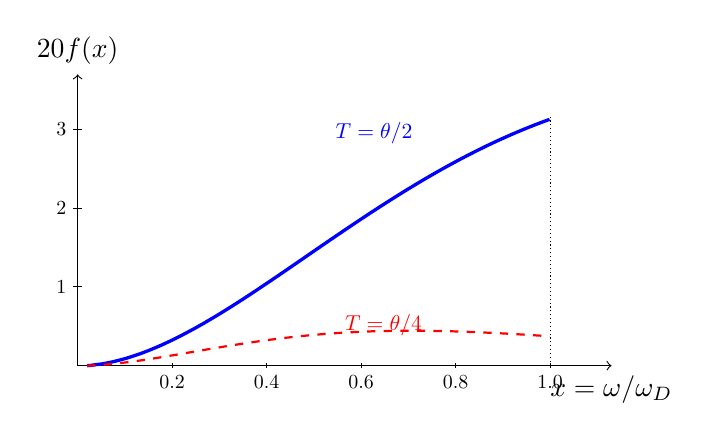
\begin{tikzpicture}[x=6.0cm,y=1.0cm]
 \draw[->] (0,0) -- (1.13,0)
  node[below] {$x=\omega/\omega_D$};
 \draw[->] (0,0) -- (0,3.7)
  node[above] {$20f(x)$};
 \foreach \x in {0.2,0.4,0.6,0.8,1.0}{
   \draw (\x,0.035) -- (\x,-0.035)
    node[below,scale=0.72] {\x};
 }
 \foreach \yy in {1,2,3}{
   \draw (0.009,\yy)--(-0.009,\yy)
   node[left,scale=0.72] {\yy};
 }
 \draw[blue,very thick]
   plot[domain=0.02:1.0,samples=100]
   (\x,{20*(\x)^3/(exp(2*\x)-1)});
 \draw[red,thick,dashed]
   plot[domain=0.02:1.0,samples=100]
   (\x,{20*(\x)^3/(exp(4*\x)-1)});
 \node[blue,anchor=west,scale=0.78] at (0.53,2.95)
  {$T=\theta/2$};
 \node[red,anchor=west,scale=0.78] at (0.55,0.52)
  {$T=\theta/4$};
 \draw[densely dotted] (1,0)--(1,3.16);
\end{tikzpicture}
\end{center}
从图及函数式均可见：较高温度的曲线
在全部$0<\omega<\omega_D$范围内更高，
且两曲线并不共享同一个谱峰位置。
\excheck 此处已经给出完整可作图的解析函数；
若发表图稿，应据函数绘制坐标图，不用任意手画频谱。

\moleculeproblem{196}{254}
估算Debye温度$\theta=330\,\mathrm K$的铜中
一个声学量子（声子）可具有的
最大能量和最大晶体准动量。
\exsolution
Debye截止角频率为
$\omega_D=k_B\theta/\hbar$，
故声子最大能量
\[
 \boxed{\varepsilon_{\max}=\hbar\omega_D=k_B\theta
 \simeq4.556\times10^{-21}\,\mathrm J
 =28.44\,\mathrm{meV}}.
\]
要求准动量不能只由能量得到，
还需要声速或晶格的截止波数。
本题给定材料是\emph{铜}，
可使用其宏观密度与摩尔质量估计原子数密度，
而无须任意指定一个声速：
\[
 n_{\rm Cu}=\frac{\rho N_A}{M}
 =\frac{8960\,\mathrm{kg/m^3}}
 {0.063546\,\mathrm{kg/mol}}N_A
 \simeq8.491\times10^{28}\,\mathrm{m^{-3}}.
\]
对三维Debye模型，三声学分支总模式数等于
$3N$，从而
\[
 3N=3\frac{V}{(2\pi)^3}\frac{4\pi k_D^3}{3},
 \qquad
 \boxed{k_D=(6\pi^2 n_{\rm Cu})^{1/3}
 \simeq1.713\times10^{10}\,\mathrm{m^{-1}}}.
\]
故模型中的最大准动量
\[
 \boxed{p_{\max}=\hbar k_D
 \simeq1.807\times10^{-24}\,\mathrm{kg\,m/s}
 =1.807\times10^{-19}\,\mathrm{g\,cm/s}}.
\]
相应的等效声速由本题给定Debye温度
\emph{反推}为
\[
 v_D=\frac{\omega_D}{k_D}
 =\frac{k_B\theta}{\hbar k_D}
 \simeq2.52\,\mathrm{km/s},
\]
并验证$p_{\max}=k_B\theta/v_D$。
\excheck 原稿曾自行取$v=3.5$km/s，
得到$1.3\times10^{-19}$g\,cm/s，
只能作为声速假设下的量级估算；
本版利用铜的原子数密度独立确定Debye截止波数，
物理条件更明确。$\hbar k_D$是
Debye连续介质模型的\emph{晶体准动量}，
并不等同于自由空间光子的动量；
原版英文“photon (acoustic quantum)”的称谓
具有混淆性，此处按声学量子即声子处理。

% === END 37-molecules-crystals-181-196.tex ===

% === BEGIN 37-molecules-crystals-197-213.tex blob e38702e5953330fb93d310baf737af9b94b0f50d ===
% 原书第六篇6.4节197--213（本节最后17题），印刷页255--256，
% PDF264--265；答案印刷348，PDF357。
\moleculeproblem{197}{255}
用零温自由电子态密度
$dn\propto\sqrt E\,dE$ 证明：
(a) 金属电子浓度为 $n$ 时最高动能 $E_F$；
(b) 零温平均电子动能与最高动能的比值。
\exsolution
三维含自旋的自由费米电子态密度为
\[
 dn=\frac{(2m_e)^{3/2}}{2\pi^2\hbar^3}
 \sqrt E\,dE,\qquad 0<E<E_F.
\]
积分得到
$n=(2m_eE_F)^{3/2}/(3\pi^2\hbar^3)$，
解得
\[
 \boxed{E_F=\frac{\hbar^2}{2m_e}(3\pi^2n)^{2/3}}.
\]
平均动能
\[
 \overline E=\frac{\int_0^{E_F}E\sqrt E\,dE}
 {\int_0^{E_F}\sqrt E\,dE}
 =\frac{(2/5)E_F^{5/2}}{(2/3)E_F^{3/2}}
 =\boxed{\frac35E_F}.
\]
\excheck 含自旋双重简并已计入态密度；
不能将费米电子平均动能误写成经典的 $3k_BT/2$。

\moleculeproblem{198}{255}
在 $T=0$ 的金属自由电子气中，
动能超过最大动能一半的电子占百分之多少？
\exsolution
零温仅填满 $0<E<E_F$ 的电子态，
其中 $dn\propto E^{1/2}\,dE$。
故
\[
 f=\frac{\int_{E_F/2}^{E_F}E^{1/2}dE}
 {\int_0^{E_F}E^{1/2}dE}
 =1-\left(\frac12\right)^{3/2}.
\]
所以
\[
 \boxed{f=1-2^{-3/2}\simeq0.6464
 \simeq64.6\%\approx65\%}.
\]
\excheck 这里积分的是\emph{态数}，
不是能量权重 $E\,dn$。

\moleculeproblem{199}{255}
钠在 $T=0$ 时费米能
$E_F=3.07\,\mathrm{eV}$，
密度 $\rho=0.97\,\mathrm{g/cm^3}$。
求平均每个钠原子贡献多少自由电子。
\exsolution
从
$E_F=\hbar^2(3\pi^2n_e)^{2/3}/(2m_e)$ 反解，
\[
 n_e=\frac1{3\pi^2}
 \left(\frac{2m_eE_F}{\hbar^2}\right)^{3/2}.
\]
钠原子数密度
$n_{\rm Na}=\rho N_A/M_{\rm Na}$，
其中 $M_{\rm Na}=22.99\,\mathrm{g/mol}$。
因此
\[
 \boxed{\nu=\frac{n_e}{n_{\rm Na}}
 =\frac{M_{\rm Na}}{3\pi^2\rho N_A}
 \left(\frac{2m_eE_F}{\hbar^2}\right)^{3/2}
 \simeq0.96\approx1}.
\]
\excheck 在模型精度下约为每原子一个自由电子；
书末简答约0.93，可能源于所采用的金属参数取值差异。

\moleculeproblem{200}{255}
把经典电子气加热到什么温度，
它的平均动能会与 $T=0$ 的铜金属自由电子的
平均动能相等？假设每个铜原子贡献一个自由电子。
\exsolution
自由电子数密度
$n=\rho_{\rm Cu}N_A/M_{\rm Cu}$。
零温平均动能 $\overline E_0=3E_F/5$，
其中
$E_F=\hbar^2(3\pi^2n)^{2/3}/(2m_e)$。
经典理想气体电子平均动能为
$3k_BT/2$，令两者相等，
\[
 \frac32k_BT=\frac35E_F
 \ \Longrightarrow\
 \boxed{T=\frac{2E_F}{5k_B}}.
\]
采用铜密度 $8.96\,\mathrm{g/cm^3}$
得到 $E_F\simeq7.04\,\mathrm{eV}$，
故
$\boxed{T\simeq3.27\times10^4\,\mathrm K
 \approx3\times10^4\,\mathrm K}$。
\excheck 该温度只是两个平均动能的\emph{数值等效温度}，
并非说铜在此温度仍保持固态金属电子气。

\moleculeproblem{201}{255}
$T=0$ 金属中自由电子浓度
$n=2.0\times10^{22}\,\mathrm{cm^{-3}}$，
金属体积 $V=1.0\,\mathrm{cm^3}$。
估算费米能附近相邻自由电子能级间隔（eV）。
\exsolution
在连续近似中粒子总数
$N(E)=V(2m_eE)^{3/2}/(3\pi^2\hbar^3)$。
费米能处态密度
$dN/dE=(3/2)(nV/E_F)$，
其中
$E_F=\hbar^2(3\pi^2n)^{2/3}/(2m_e)$。
因此平均相邻\emph{电子态}的能距
\[
 \boxed{\delta E\simeq
 \left(\frac{dN}{dE}\right)^{-1}_{E_F}
 =\frac{2E_F}{3nV}
 =\frac{\pi^2\hbar^2}{m_eV}(3\pi^2n)^{-1/3}}.
\]
将 $n=2.0\times10^{28}\,\mathrm{m^{-3}}$、
$V=10^{-6}\,\mathrm{m^3}$ 代入，
得到 $E_F\simeq2.687\,\mathrm{eV}$ 及
\[
\boxed{\delta E\simeq8.96\times10^{-23}\,\mathrm{eV}
\sim10^{-22}\,\mathrm{eV}}.
\]
\excheck 用 $2E_F/(3nV)$ 对最终幂式反代，
得到前因子应为 $\pi^2\hbar^2/(m_eV)$，而非
$\hbar^2/(3m_eV)$；先前形式少了 $3\pi^2$ 倍。
此定义计入每个空间轨道的两个自旋态；
若讨论\emph{不同能量值}而非电子态，
简并与边界几何会改变系数。原书给约
$2\times10^{-22}\,\mathrm{eV}$，与该量级一致。

\moleculeproblem{202}{255}
依据零温自由电子态密度，
(a) 推导电子速率分布 $dn_v$；
(b) 求平均速率与最大费米速率之比。
\exsolution
令 $E=m_ev^2/2$，
$0\le v\le v_F$，
由 $dn\propto\sqrt E\,dE$ 与
$dE=m_ev\,dv$，故
\[
 \boxed{dn_v=\frac{m_e^3}{\pi^2\hbar^3}v^2\,dv},
 \qquad
 \boxed{f(v)=\frac3{v_F^3}v^2},
 \quad 0<v<v_F.
\]
平均速率为
\[
 \overline v=\int_0^{v_F}vf(v)dv
 =\frac{3}{v_F^3}\frac{v_F^4}{4},
 \quad \boxed{\frac{\overline v}{v_F}=\frac34}.
\]
\excheck 零温下速率并非全部为零；
费米简并使电子填充从0到费米动量的态。

\moleculeproblem{203}{255}
从三维自由电子态密度导出：
在 $T=0$ 金属中，
以德布罗意波长 $\lambda$ 计数的电子分布。
\exsolution
含自旋简并的动量空间态密度满足
\[
 dn=\frac{2}{(2\pi\hbar)^3}\,4\pi p^2\,dp
 =\frac{p^2}{\pi^2\hbar^3}\,dp.
\]
利用 $p=h/\lambda=2\pi\hbar/\lambda$，
$|dp/d\lambda|=2\pi\hbar/\lambda^2$，得
\[
 \boxed{dn_\lambda=
 \frac{p^2}{\pi^2\hbar^3}
 \left|\frac{dp}{d\lambda}\right|d\lambda
 =\frac{8\pi}{\lambda^4}\,d\lambda},
 \quad \lambda\ge\lambda_F=h/p_F.
\]
\excheck 虽然分布不显含电子质量，
但是允许的最低波长
$\lambda_F=h/\sqrt{2m_eE_F}$包含材料电子浓度。

\moleculeproblem{204}{255}
零温金属钠的自由电子浓度
$n=2.5\times10^{22}\,\mathrm{cm^{-3}}$。
用理想气体动量通量表达式估算电子简并压强。
\exsolution
各向同性粒子气压强
$p=(1/3)n\langle pv\rangle$。
非相对论电子 $pv=2E$，故
\[
 p=\frac23n\overline E
 =\frac23n\frac35E_F=\frac25nE_F,
\]
\[
 \boxed{p=\frac{\hbar^2}{5m_e}(3\pi^2)^{2/3}n^{5/3}}.
\]
将 $n=2.5\times10^{28}\,\mathrm{m^{-3}}$ 代入，
得
$\boxed{p\simeq5.1\times10^9\,\mathrm{Pa}
 \approx5.0\times10^4\,\mathrm{atm}}$。
\excheck 零温量子简并压强不为零，
不同于经典 $p=nk_BT$ 的简单零温外推。

\moleculeproblem{205}{255}
电子管阴极温度从 $T=2000\,\mathrm K$
升高 $\Delta T=1.0\,\mathrm K$，
饱和发射电流增大 $\eta=1.4\%$。
求阴极材料逸出功。
\exsolution
由 Richardson--Dushman 关系
$I_s=C T^2e^{-W/(k_BT)}$，
对数微分
\[
 \frac{\Delta I_s}{I_s}\simeq
 \left(\frac2T+\frac W{k_BT^2}\right)\Delta T.
\]
故
\[
 \boxed{W=k_BT\left[
 \frac{\eta T}{\Delta T}-2\right]}.
\]
代 $\eta=0.014$ 得
$\boxed{W\simeq4.48\,\mathrm{eV}\approx4.5\,\mathrm{eV}}$。
\excheck $\eta$ 是相对增长的无量纲数 $0.014$，
而不是数字1.4。

\moleculeproblem{206}{255}
动能 $T=135\,\mathrm{eV}$ 的电子射入金属钠，
求其电子波的折射率。
设每钠原子贡献一个自由电子。
\exsolution
电子由真空进入金属时，
可用内势能降低 $U_0=E_F+W$，
其中 $E_F$ 是零温金属费米能，
$W$ 为金属表面逸出功。
动量分别
$p_{\rm out}=\sqrt{2m_eT}$、
$p_{\rm in}=\sqrt{2m_e(T+U_0)}$，故
\[
 \boxed{n_e=\frac{\lambda_{\rm out}}{\lambda_{\rm in}}
 =\sqrt{1+\frac{U_0}{T}}}.
\]
由 $n_{\rm Na}=\rho N_A/M_{\rm Na}$、
每原子一电子，
$E_F\simeq3.15\,\mathrm{eV}$。
采用钠逸出功 $W\simeq2.3\,\mathrm{eV}$
给 $U_0\simeq5.45\,\mathrm{eV}$，所以
$\boxed{n_e\simeq1.020\approx1.02}$。
\excheck 题面未另给逸出功，
故明确引用表值；数值近似
$n_e\simeq1+U_0/(2T)$ 而非 $1+U_0/T$。

\moleculeproblem{207}{255}
本征半导体从 $T_1=300\,\mathrm K$
升温到 $T_2=400\,\mathrm K$ 时，
电导率增为原来的 $\eta=5.0$ 倍。
忽略迁移率温度变化，
求形成电子--空穴对的最低能量。
\exsolution
本征载流子浓度的主指数为
$n_i\propto\exp[-E_g/(2k_BT)]$，
电导率同样满足
$\sigma\propto e^{-E_g/(2k_BT)}$。
于是
\[
 \ln\eta=\frac{E_g}{2k_B}
 \left(\frac1{T_1}-\frac1{T_2}\right),
\quad
 \boxed{E_g=\frac{2k_BT_1T_2}{T_2-T_1}\ln\eta}.
\]
代入
$\boxed{E_g\simeq0.333\,\mathrm{eV}}$。
\excheck 电子--空穴对的形成能与带隙 $E_g$
一致；电导率指数中有 $1/2$ 是因为本征
电子、空穴各贡献一半的激发熵关系。

\moleculeproblem{208}{255}
本征锗的低温光电截止波长为
$\lambda_{\rm th}=1.7\,\mu\mathrm m$。
估算室温时电阻率温度系数
$\alpha=(1/\rho)d\rho/dT$。
\exsolution
低温阈值对应带隙
$E_g=hc/\lambda_{\rm th}$。
忽略迁移率的温度依赖，
本征电阻率
$\rho(T)\propto e^{E_g/(2k_BT)}$。
因此
\[
 \boxed{\alpha=\frac{d\ln\rho}{dT}
 =-\frac{E_g}{2k_BT^2}
 =-\frac{hc}{2\lambda_{\rm th}k_BT^2}}.
\]
代 $T=300\,\mathrm K$，得
$\boxed{\alpha\simeq-0.047\,\mathrm{K^{-1}}
 \approx-0.05\,\mathrm{K^{-1}}}$。
\excheck 本征半导体升温载流子浓度增加，
电阻率下降，故温度系数为负。

\moleculeproblem{209}{256}
原图6.11以 $\ln\sigma$ 为纵轴，
$T^{-1}$ 为横轴，展示某 n 型半导体的
高温本征段与低温施主激活段。
根据两段直线斜率求禁带宽度和施主能级激活能。
\exsolution
本征高温段满足
$\ln\sigma=\mathrm{const}-E_g/(2k_BT)$，
因此曲线斜率
$s_i=d(\ln\sigma)/d(1/T)=-E_g/(2k_B)$。
低温施主热激活段
$\ln\sigma=\mathrm{const}-E_d/(2k_BT)$，
同理 $s_d=-E_d/(2k_B)$。
故
\[
 \boxed{E_g=-2k_Bs_i},\qquad
 \boxed{E_d=-2k_Bs_d}.
\]
由原图两段斜率约为
$s_i\simeq-7.0\times10^3\,\mathrm K$、
$s_d\simeq-3.5\times10^2\,\mathrm K$，
得到
$\boxed{E_g\simeq1.2\,\mathrm{eV},\quad
 E_d\simeq0.06\,\mathrm{eV}}$。
\excheck 原图横轴仅标 $T^{-1}$ 及1--4刻度，
实际读数需按常见 $10^{-3}\,\mathrm{K^{-1}}$
尺度理解；若按 $1\,\mathrm{K^{-1}}$ 读，
无法得到合理半导体能隙。源图隐含标度应在校订图中注明。

\moleculeproblem{210}{256}
本征半导体暗态电阻率
$\rho=50\,\Omega\cdot\mathrm{cm}$；
照光后降到
$\rho_1=40\,\Omega\cdot\mathrm{cm}$。
关光 $t=8\,\mathrm{ms}$ 后
变为 $\rho_2=45\,\Omega\cdot\mathrm{cm}$。
求非平衡电子与空穴平均寿命。
\exsolution
光生超额电导随关光时间按
$\Delta\sigma(t)=\Delta\sigma(0)e^{-t/\tau}$ 衰减。
$\sigma=1/\rho$，
故
\[
 e^{-t/\tau}=
 \frac{1/\rho_2-1/\rho}{1/\rho_1-1/\rho}
 =\frac{(\rho-\rho_2)\rho_1}
 {(\rho-\rho_1)\rho_2}.
\]
反解
\[
 \boxed{\tau=\frac t{
 \ln[(\rho-\rho_1)\rho_2/((\rho-\rho_2)\rho_1)]}
 \simeq9.87\,\mathrm{ms}\approx0.010\,\mathrm s}.
\]
\excheck 指数衰减的对象是光生\emph{超额电导}，
不是简单的电阻率差 $\rho(t)-\rho$。

\moleculeproblem{211}{256}
p型半导体板宽 $h=10\,\mathrm{mm}$、
长 $l=50\,\mathrm{mm}$，
磁感应强度 $B=5.0\,\mathrm{kG}$，
纵向电压 $V=10\,\mathrm V$、
霍尔电压 $V_H=50\,\mathrm{mV}$，
电阻率 $\rho=2.5\,\Omega\cdot\mathrm{cm}$。
求空穴数密度和迁移率。
\exsolution
纵向电场 $E_x=V/l$，
电流密度 $j=E_x/\rho=V/(\rho l)$。
霍尔电场 $E_H=V_H/h$。
单一空穴载流子的霍尔平衡
$E_H=jB/(ne)$，故
\[
 \boxed{n=\frac{hBV}{e\,l\rho V_H}}.
\]
迁移率由 $\sigma=ne\mu_h=1/\rho$ 给
\[
 \boxed{\mu_h=\frac1{ne\rho}
 =\frac{lV_H}{hBV}}.
\]
把 $B=0.50\,\mathrm T$、$\rho=0.025\,\Omega\mathrm m$
代入，
\[
 \boxed{n\simeq5.0\times10^{15}\,\mathrm{cm^{-3}},
 \quad\mu_h\simeq0.050\,\mathrm{m^2/(V\,s)}}.
\]
\excheck 电阻率 $2.5\,\Omega\cdot\mathrm{cm}$
必须换成 $0.025\,\Omega\mathrm m$。

\moleculeproblem{212}{256}
在本征锗中，外磁场
$B=5.0\,\mathrm{kG}$；
霍尔横向电场强度比纵向电场
低 $\eta=10$ 倍。求电子、空穴迁移率之差。
\exsolution
本征半导体电子与空穴浓度相等。
低磁场双载流子模型
\[
 R_H=\frac{\mu_h^2-\mu_e^2}
 {en(\mu_h+\mu_e)^2}
 =\frac{\mu_h-\mu_e}{en(\mu_h+\mu_e)}.
\]
电导率
$\sigma=en(\mu_h+\mu_e)$，因此
\[
 \frac{E_H}{E_x}=R_H\sigma B
 =(\mu_h-\mu_e)B.
\]
取绝对值及 $E_H/E_x=1/\eta$，
\[
 \boxed{|\mu_h-\mu_e|=\frac1{\eta B}
 =\frac1{10\times0.50}
 =0.20\,\mathrm{m^2/(V\,s)}}.
\]
\excheck 在本征样品中
不能套用单载流子的 $R_H=1/(ne)$，
必须使用双载流子霍尔表达式。

\moleculeproblem{213}{256}
某半导体未观察到霍尔效应，
其电子迁移率是空穴迁移率的
$\eta=2.0$ 倍。
求空穴数密度与导带电子数密度之比。
\exsolution
双载流子霍尔系数
\[
 R_H=\frac{n_h\mu_h^2-n_e\mu_e^2}
 {e(n_h\mu_h+n_e\mu_e)^2}.
\]
若霍尔效应抵消，$R_H=0$，
故
$n_h\mu_h^2=n_e\mu_e^2$，
从而
\[
 \boxed{\frac{n_h}{n_e}=
 \left(\frac{\mu_e}{\mu_h}\right)^2
 =\eta^2=4}.
\]
\excheck 霍尔效应为零不说明无载流子，
而是电子和空穴的霍尔贡献恰好相互抵消。
% === END 37-molecules-crystals-197-213.tex ===
